
%% NAT Visualisierungen
\begin{figure}[H]
  \centering
  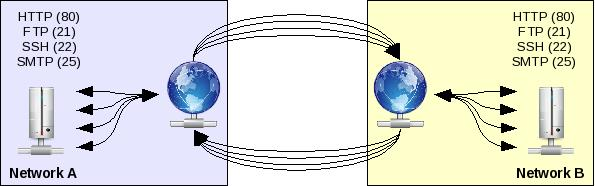
\includegraphics[width=0.6\linewidth]{images/theorie/nat-source}
  \caption[Anzahl NAT-Regeln bei zwei Netzwerken]{Beispiel f\"ur die Anzahl NAT-Regeln bei zwei Netzwerken mit jeweils einem Host, welche je vier Dienste \"uberwacht haben wollen. Beide NAT-Firewalls m\"ussen je vier Regeln definiert haben, um die Anfragen durch zu leiten.}
  \label{fig:nat-source}
\end{figure}

\begin{figure}[H]
  \centering
  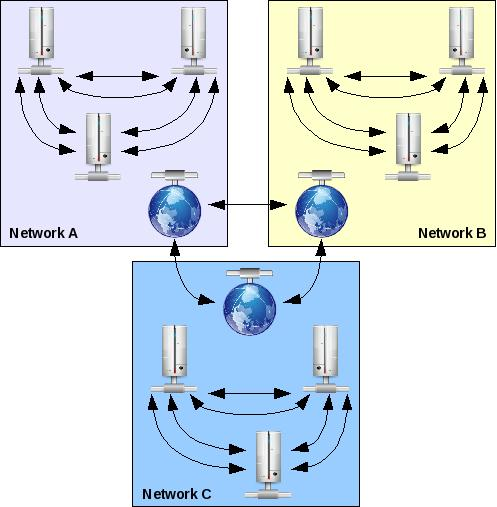
\includegraphics[width=0.6\linewidth]{images/theorie/nat-verteilt}
  \caption[Anzahl NAT-Regeln bei einer verteilten \"Uberwachung]{Beispiel f\"ur die Anzahl NAT-Regeln bei einer verteilten \"Uberwachung. Die NAT-Boxen m\"ussen jeweils nur eine Regel pro entferntem Netzwerk definiert haben, da dieses als Ganzes \"uberwacht wird und nicht jedes System einzeln.}
  \label{fig:nat-verteilt}
\end{figure}


%% Hypercube Visualisierungen
\begin{figure}[H]
  \centering
  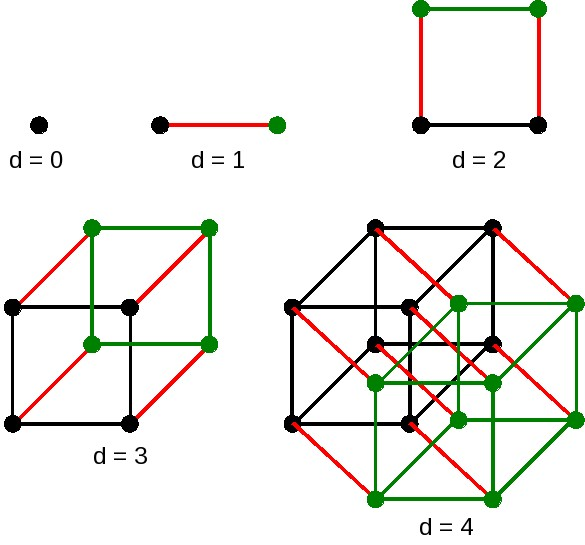
\includegraphics[width=0.6\linewidth]{images/theorie/hyper-sample}
  \caption[Hypercubes von Dimension 0 bis 4]{Hypercubes von Dimension $d=0$ bis $d=4$. Die Erstellung geschieht jeweils durch eine Verschiebung (gr\"un) des vorherigen Hypercubes in eine neue Dimension sowie dem Verbinden (rot) der jeweils gleichen Eckpunkte miteinander.}
  \label{fig:hyper-sample}
\end{figure}

\begin{figure}[H]
  \centering
  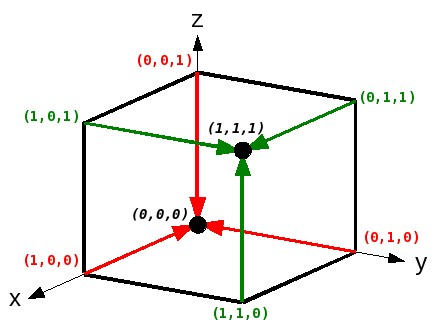
\includegraphics[width=0.6\linewidth]{images/theorie/hyper-hamming-4}
  \caption[Hamming-Distanz bei einem Hypercube zur Nummerierung der Nodes]{Die Nummerierung mit der Hamming-Distanz geschieht bei einem W\"urfel durch die Zuweisung der Werte $(0,0,0)$ und $(1,1,1)$ auf zwei gegen\"uberliegenden Ecken und anschliessend dem Verschieben der $1$ resp. der $0$ im Uhrzeigersinn auf den umliegenden Ecken.}
  \label{fig:hyper-hamming-num}
\end{figure}

%% SNMP Samples
\begin{figure}[H]
  \centering
  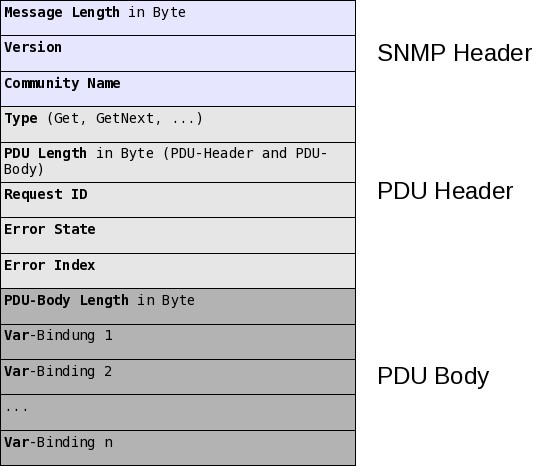
\includegraphics[width=0.8\linewidth]{images/theorie/snmp-packet}
  \caption[Aufbau eines SNMP-Pakets]{Aufbau eines SNMP-Pakets. Die in der MIB definierten Daten werden als MO, also Key-Value Paar, im PDU-Body nacheinander angegeben. Achtung: Der PDU-Header bei einem TRAP-Paket weist andere Daten auf, der PDU-Body ist jedoch gleich aufgebaut.}
  \label{fig:snmp-packet}
\end{figure}

\begin{figure}[H]
  \lstset{morecomment=[l]{--}}
  \begin{lstlisting}[label=code:mib-inetAddress,caption={[SNMP-MIB einer IPv4-Adresse]MIB-Definition f\"ur eine IP-Adresse - definiert in der INET-ADDRESS-MIB}]
InetAddressIPv4 ::= TEXTUAL-CONVENTION
    DISPLAY-HINT "1d.1d.1d.1d"
    STATUS       current
    DESCRIPTION
        "Denotes a generic Internet address...."
    SYNTAX       OCTET STRING (SIZE (4))
  \end{lstlisting}
  \label{code:mib-ipAddress}
\end{figure}


%% Code-Fragmente: Praktische Umsetzung
\begin{figure}[H]
 \lstset{language=[ISO]C++}
 \begin{lstlisting}[label=alg:praxis-basis-netservice,caption={[Datenstruktur Helper.NetService]Die Datenstruktur Helper.NetService wird verwendet um die Verf\"ugbarkeit eines Dienstes, respektive eines Monitoring-Modules, auf einem System zu definieren.}]
  public struct NetService {
    public string host;
    public string monitor;
    public string network;
    public bool available;
    public string to_string() {
      return @"host: $host\nmonitor: $monitor\nnetwork:"+
              "$network\navailable: %s".printf(available?"Yes":"No");
    }
  }

 \end{lstlisting}
\end{figure}

\begin{figure}[H]
 \lstset{language=[ISO]C++}
 \begin{lstlisting}[label=alg:praxis-basis-kernel-msg,caption={[Asynchrone MessageQueue und Datentyp RequestData]Die asynchrone Queue, typisiert auf \texttt{RequestData}, beinhaltet alle Nachrichten\index{Nachricht}, welche nacheinander abgearbeitet werden. Die Nachrichten werden durch die Klasse \texttt{RequestData} definiert, wobei das Kommando immer angegeben werden muss, die Daten sind jedoch optional.\index{MessageQueue}\index{RequestData}}]
  AsyncQueue<RequestData> request_queue;

  class RequestData {
    public string command {get; private set;}
    public string data {get; private set;}
    public RequestData(string cmd, string? args="") {
      command = cmd;
      data = args;
    }
  }
 \end{lstlisting}
\end{figure}

\begin{figure}[H]
 \lstset{language=[ISO]C++}
 \begin{lstlisting}[label=alg:praxis-basis-imainmodule,caption={[Interface: IMainModule]Das Haupt-Interface von Plugins beinhaltet nur Methoden zur Registrierung des Modul-Containers sowie Properties f\"ur den Identifier und den Pfad, welche in der Einstiegsfunktion des Plugins schon definiert sind.}]
interface IMainModule : Object {
  public abstract void setRegistrar(PluginRegistrar registrar);
  public abstract string identifier { public get; public set; }
  public abstract string path { public get; public set; }
}
 \end{lstlisting}
\end{figure}

\begin{figure}[H]
 \lstset{language=[ISO]C++}
 \begin{lstlisting}[label=alg:praxis-basis-icommodule,caption={[Interface: ICommModule]Das Interface eines Netzwerk- und BUS-Modules. Die Signale \texttt{onError}, \texttt{onData} und \texttt{onComplete} k\"onnen auf mehrere unterschiedliche Empf\"anger gebunden werden.}]
interface ICommModule : IMainModule {
  public signal void onError(string ip, string data, int code);
  public signal void onData(string ip, string data, bool more);
  public signal void onComplete(string ip, string[] data,
                                int code);

  public abstract async void send(string? data="");
  public abstract void setParam(string key, string value);
  public abstract string getParam(string key);
}
 \end{lstlisting}
\end{figure}

\begin{figure}[H]
 \lstset{language=[ISO]C++}
 \begin{lstlisting}[label=alg:praxis-basis-imonitormodule,caption={[Interface: IMonitorModule]Das Interface eines \"Uberwachungsmoduls besteht haupts\"achlich aus der Methode \texttt{monitor()}, welche asynchron definiert ist, um nicht auf eine R\"uckmeldung warten zu m\"ussen. Die Properties \texttt{timeout}, \texttt{next\_run} und \texttt{running} dienen zur Pr\"ufung, ob ein Modul aktuell eine Pr\"ufung durchf\"uhrt oder nicht, sowie um den Zeitpunkt der n\"achsten Pr\"ufung zu berechnen.}]
interface IMonitorModule : IMainModule {
  public abstract int timeout { public get; public set;
                                default=1; }
  public abstract long next_run { public get; public set;
                                  default=0; }
  public abstract bool running { public get; public set;
                                 default=false; }

  public abstract void setParam(string key, string value);
  public abstract string getParam(string key);

  public async abstract void monitor();
}
 \end{lstlisting}
\end{figure}

\begin{figure}[H]
 \lstset{language=[ISO]C++}
 \begin{lstlisting}[label=alg:praxis-basis-idatamodule,caption={[Interface: IDataModule]Das Interface eines Datenmodules beinhaltet Methoden zum Auslesen wie auch zum Schreiben von Daten. Zus\"atzlich sind noch verschiedene Datentypen, Konstanten und Strukturen definiert, welche bei der Initialisierung und der Datenbehandlung gebraucht werden. Die zus\"atzlichen Konstanten, Strukturen und Datentypen werden hier nur exemplarisch dargestellt.}]
interface IDataModule : IMainModule {
  public abstract IDataModule.DataType data_type { public get;
                                                   public set; };
  public abstract bool open(string db_name);
  public abstract bool select(string? fields="*",
                              string? groupBy="");
  public abstract void setWhere(string field, string value);
  public abstract bool hasNext();
  public abstract IDataModule.DataSet[] getCurrent();
  public abstract string getValue(string field);
  public abstract bool save(IDataModule.DataSet[] values,
                            IDataModule.DataSet[]? where=null);
  public abstract bool delete(IDataModule.DataSet[] where);
  public abstract bool empty();

  public struct DataSet { ... };
  public struct SchemaField { ... };
  public enum DataType { ... };
  public enum SchemaFieldType { ... };

  public const string TABLE_XX = "Tablename";
  public const string[] SCHEMA_XX = {
      "name,type,length,defval,primkey",
      "..."
  };
}
 \end{lstlisting}
\end{figure}

\begin{figure}[H]
 \lstset{language=[ISO]C++}
 \begin{lstlisting}[label=alg:praxis-basis-ialertmodule,caption={[Interface: IAlertModule]Das Interface eines Alert-Modules ist sehr einfach und besitzt eigentlich nur eine Methode um einen Alert zu senden, ein Signal f\"ur die \"Ubermittlungsbest\"atigung und eine Methode zur Konfiguration des Modules.}]
interface IAlertModule : IMainModule {
  public signal void onSent(string[] recp, string uid,
                            int state, string? msg="");
  public abstract void setParam(string key, string value);
  public abstract async void send(string subject,
                                  string short_message,
                                  string message,
                                  string[]? attach=null);
}
 \end{lstlisting}
\end{figure}

\begin{figure}[H]
 \lstset{language=[ISO]C++}
 \begin{lstlisting}[label=alg:praxis-basis-iremotemodule,caption={[Interface: IRemoteModule]Ein Remote-API Modul muss lediglich bei der Instanzierung konfiguriert werden. Anschliessend wird \"uber die Methode \texttt{startThread()} ein eigener Thread gestartet, welcher die komplette Kommunikation mit den Clients \"ubernimmt. Der Konformit\"at zuliebe wurde die Methode \texttt{parseRequest(string? data="`"')} dennoch in das Interface aufgenommen.}]
interface IRemoteModule : IMainModule {
  public abstract void startThread();
  public abstract void setParam(string key, string value);
  public abstract void parseRequest(string? data="");
}
 \end{lstlisting}
\end{figure}


%% Remote-System Kommunikation
\begin{table}[H]
\centering
\begin{tabular}{c|l|p{7.3cm}}
 \toprule
 Kommando & Daten & Beschreibung\\
 \midrule
 discover & \texttt{IP-ADDRESS MASK} & Startet die automatische Suche nach Systemen im angegebenen Netzwerk.\\
 \midrule
 testdata & \texttt{IP-ADDRESS MASK NUM} & Erstellt \texttt{NUM} Pseudo-Systeme in der Datenbank im angegebenen Netzwerk f\"ur verschiedene Tests.\\
 \midrule
 testdata & - & Ohne Daten werden alle Pseudo-Systeme aus der Netzwerk- und der Hosts-Tabelle entfernt, nicht jedoch aus dem Monitoring.\\
 \midrule
 monitor & \texttt{IP-ADDRESS[ ...]} & Teilt dem System mit, dass es f\"ur die \"Uberwachung aller angegebenen IP-Adressen zust\"andig ist.\\
 \midrule
 synchronize & - & Ohne Daten wird die Synchronisation gestartet.\\
 \midrule
 synchronize & \texttt{netw ($\backslash$t A.B.C.D/MASK)+} & Durch das Prefix "`netw"' sowie der Angabe aller Netzwerke als Tabulator getrennte Liste, werden alle Netzwerke aus der Datenbank durch die angegebenen ersetzt.\\
 \midrule
 synchronize & \texttt{host $\backslash$t IP ($\backslash$t MOD;KEY;VAL)+} & Durch das Prefix "`host"' sowie der Angabe einer IP-Adresse werden alle Hosts-Eintr\"age aus der Datenbank entfernt. Die Tabulator getrennte Liste, bestehend aus den Angaben "`ModuleName;Key-Name;Wert"', wird anschliessend verwendet um neue Datens\"atze zu generieren.\\
 \midrule
 alert & \texttt{MODULE IP-ADDRESS GUID} & Teilt dem System mit, dass das gegebene Modul bei dem System fehlgeschlagen und ein Alert mit der GUID versendet worden ist.\\
 \midrule
 rebuild & - & Verkn\"upft alle Systeme zu einem neuen \"Uberwachungs-Netzwerk.\\
 \midrule
 exit & - & Beendet das System.\\
 \bottomrule
\end{tabular}
\caption[Kommandos f\"ur entfernte Systeme]{Kommandos und Daten, die ein entferntes System senden kann.}
\label{tbl:praxis-basis-kernel-remote}
\end{table}


%% Datenbank-Tabellen
\begin{table}[H]
\centering
\begin{tabular}{l|c|c|l|c|p{8cm}}
 \toprule
 Feld & Typ & L\"ange & Std. & PK & Beschreibung\\
 \midrule
 section & string & 20 & - & No & Bereich des Parameter\\
 \midrule
 key & string & 50 & - & No & Parameter Name\\
 \midrule
 value & text & - & - & No & Parameter Wert\\
 \bottomrule
\end{tabular}
\caption[Datenbank-Tabelle: CONF]{Datenbank \texttt{CONF}: Konfiguration verschiedener Systembereiche.}
\label{tbl:praxis-basis-data-table_conf}
\end{table}
% SCHEMA_CONF = {"section,string,20,,0", "key,string,50,,0", "value,text,,,0"};

\begin{table}[H]
\centering
\begin{tabular}{l|c|c|l|c|p{7cm}}
 \toprule
 Feld & Typ & L\"ange & Std. & PK & Beschreibung\\
 \midrule
 network & string & 39 & - & No & Netzwerk (IP-)Adresse\\
 \midrule
 mask & int & 2 & 0 & No & Subnetmaske\\
 \midrule
 discoverable & int & 1 & 0 & No & Das Netzwerk kann untersucht werden 1=ja, 0=nein\\
 \midrule
 vpn\_gateway & string & 39 & - & No & Adresse des VPN-Gateway in dieses Netzwerk\\
 \midrule
 vpn\_user & string & 20 & - & No & Benutzer f\"ur die OpenVPN-Verbindung\\
 \midrule
 vpn\_pass & string & 20 & - & No & Passwort f\"ur die OpenVPN-Verbindung\\
 \midrule
 is\_test & int & 1 & 0 & No & Ist auf 1, wenn es sich um ein Pseudo-Test-Netzwerk handelt\\
 \bottomrule
\end{tabular}
\caption[Datenbank-Tabelle: NETWORKS]{Datenbank \texttt{NETWORKS}: Definition der verschiedenen Netzwerke, die \"uberwacht werden.}
\label{tbl:praxis-basis-data-table_netw}
\end{table}
% SCHEMA_NETWORKS = {"network,string,39,,0", "mask,int,2,0,0", "discoverable,int,1,0,0", "vpn_gateway,string,20,,0", "vpn_user,string,20,,0", "vpn_pass,string,20,,0", "is_test,int,1,0,0"};

\begin{table}[H]
\centering
\begin{tabular}{l|c|c|l|c|p{8cm}}
 \toprule
 Feld & Typ & L\"ange & Std. & PK & Beschreibung\\
 \midrule
 host & string & 39 & - & No & Adresse des zu \"uberwachenden Systems\\
 \midrule
 module & string & 20 & - & No & Modulname\\
 \midrule
 key & string & 50 & - & No & Parameter-Name\\
 \midrule
 value & text & - & - & No & Parameter-Wert\\
 \midrule
 is\_test & int & 1 & 0 & No & Ist auf 1, wenn es sich um ein Pseudo-Test-Host handelt\\
 \bottomrule
\end{tabular}
\caption[Datenbank-Tabelle: HOSTS]{Datenbank \texttt{HOSTS}: Alle Systeme und \"Uberwachngs-Dienste sowie Konfigurationsparameter, welche bei einem Host-Discovery gefunden wurden.}
\label{tbl:praxis-basis-data-table_hosts}
\end{table}
% SCHEMA_HOSTS = {"host,string,39,,0", "module,string,20,,0", "key,string,50,,0", "value,text,,,0", "is_test,int,1,0,0"};

\begin{table}[H]
\centering
\begin{tabular}{l|c|c|l|c|p{8cm}}
 \toprule
 Feld & Typ & L\"ange & Std. & PK & Beschreibung\\
 \midrule
 host & string & 39 & - & No & Adresse des zu \"uberwachenden Systems\\
 \midrule
 module & string & 20 & - & No & Modulname\\
 \midrule
 key & string & 50 & - & No & Parameter-Name\\
 \midrule
 value & text & - & - & No & Parameter-Wert\\
 \bottomrule
\end{tabular}
\caption[Datenbank-Tabelle: MODULES]{Datenbank \texttt{MODULES}: Alle Systeme und \"Uberwachungs-Dienste sowie deren Parameter.}
\label{tbl:praxis-basis-data-table_modules}
\end{table}
% SCHEMA_MODULES = {"module,string,20,,0", "host,string,39,,0", "key,string,50,,0", "value,text,,,0"};

\begin{table}[H]
\centering
\begin{tabular}{l|c|c|l|c|p{8cm}}
 \toprule
 Feld & Typ & L\"ange & Std. & PK & Beschreibung\\
 \midrule
 host & string & 39 & - & No & Adresse des zu \"uberwachenden Systems\\
 \midrule
 module & string & 20 & - & No & Modulname\\
 \midrule
 state & uint & 4 & 0 & No & Status\\
 \midrule
 time & uint & 11 & 0 & No & Timestamp\\
 \midrule
 message & text & - & - & No & Nachricht/Daten\\
 \bottomrule
\end{tabular}
\caption[Datenbank-Tabelle: MONITOR]{Datenbank \texttt{MONITOR}: Alle Monitoring-Nachrichten.}
\label{tbl:praxis-basis-data-table_monitor}
\end{table}
% SCHEMA_MONITOR = {"module,string,20,,0", "host,string,39,,0", "state,uint,4,0,0", "time,uint,11,0,0", "message,text,,,0"};

\begin{table}[H]
\centering
\begin{tabular}{l|c|c|l|c|p{7.5cm}}
 \toprule
 Feld & Typ & L\"ange & Std. & PK & Beschreibung\\
 \midrule
 host & string & 39 & - & No & Adresse des zu \"uberwachenden Systems\\
 \midrule
 module & string & 20 & - & No & Modulname\\
 \midrule
 subject & string & 20 & - & No & Betreff der Nachricht\\
 \midrule
 short & string & 160 & - & No & Kurze Meldung\\
 \midrule
 message & text & - & - & No & Ausf\"uhrliche Meldung\\
 \midrule
 uid & string & 64 & - & No & Die GUID des Alerts\\
 \bottomrule
\end{tabular}
\caption[Datenbank-Tabelle: ALERT]{Datenbank \texttt{ALERT}: Alle Alert-Nachrichten, die durch das aktuelle System versandt worden w\"aren. Es werden auch die Nachrichten gespeichert, welche aufgrund des Timeouts nicht versendet worden sind.}
\label{tbl:praxis-basis-data-table_alert}
\end{table}
% SCHEMA_ALERT = {"module,string,20,,0", "host,string,39,,0", "subject,string,20,,0", "short,string,160,,0", "message,text,,,0", "attachment,blob,,,0"};

\begin{table}[H]
\centering
\begin{tabular}{l|c|c|l|c|p{7.5cm}}
 \toprule
 Feld & Typ & L\"ange & Std. & PK & Beschreibung\\
 \midrule
 host & string & 39 & - & No & Adresse des zu \"uberwachenden Systems\\
 \midrule
 module & string & 20 & - & No & Modulname\\
 \midrule
 tstamp & uint & 11 & 0 & No & Zeitstempel des aktuellen Systems\\
 \midrule
 sent\_host & string & 39 & - & No & Adresse des Systems, welches die Nachricht versandt hat\\
 \midrule
 uid & string & 64 & - & No & Die GUID des Alerts\\
 \bottomrule
\end{tabular}
\caption[Datenbank-Tabelle: ALERT\_SENT]{Datenbank \texttt{ALERT\_SENT}: Alle Alert-Nachrichten, welche von anderen und diesem System versandt worden sind. Dient zur Pr\"ufung, ob eine Benachrichtigung versendet werden soll oder nicht.}
\label{tbl:praxis-basis-data-table_alertsent}
\end{table}
% SCHEMA_ALERT_SENT = {"module,string,20,,0", "host,string,39,,0", "tstamp,uint,11,0,0", "sent_host,string,39,,0"};

% Pseudo-Konfiguration der TechDemo
\begin{table}[H]
\centering
\begin{tabular}{l|l|p{8cm}}
 \toprule
 Key & Value & Beschreibung\\
 \midrule
 to\_list & em@il.dom,em@il.dom & Kommaseparierte Liste mit allen EMail-Adressen, an welche ein Alert versendet werden soll\\
 \midrule
 mail\_from & em@il.dom & EMail-Adresse des Alert-Absenders\\
 \midrule
 host & IP-Address | DNS & IP-Adresse oder DNS-Name des MX-Servers\\
 \midrule
 auth\_method & plain | login & Authentifizierungs-Methode. Aktuell werden LOGIN und PLAIN unterst\"utzt\\
 \midrule
 username & em@ail.com & Benutzername f\"ur Relaying\\
 \midrule
 password & abc & Passwort zum obigen Benutzernamen\\
 \bottomrule
\end{tabular}
\caption[Datei dummy\_alert\_config.txt]{Die Datei "`dummy\_alert\_config.txt"' im data-Ordner beinhaltet aktuell die Konfiguration des EMail-Alert-Modules. Key und value werden durch einen Doppelpunkt getrennt: "`host:1.2.3.4"'.}
\label{tbl:praxis-install-dummyalertconf}
\end{table}


